\item{\textbf{Station Keeping}}
\begin{itemize}
\item{\textbf{Description of mission}}


As the WRSC rules described, the objective of the station keeping contest is to evaluate controlled sailing in a limited region with time constraints. Each boat must start outside a 45 m x 45 m box, marked by four buoys. In the team slot time, the boat must enter the box. The boat shall leave the box at a time as close as possible to 5 minutes after entering the box. Boats fulfilling the entry and exit criteria are awarded points based on the following formula:
\begin{lstlisting}
P = max (0, 10 - |Tenter + 300 - Tleave|/10)
Where: Tenter is the timestamp when the boat first enters the box and Tleave is the timestamp
\end{lstlisting}
when the boat first leaves the box. If the boat enters and leaves the box several times, any leave timestamps within ten seconds from Tenter are ignored. All timestamps are given in seconds.


\item{\textbf{algorithm for Station Keeping}}


In general, the aim of station keeping is letting the boat stay 300s exactly in a square(ideally), or more generally stay in a polygon. So the key point of calculating the score is checking whether the position of boat is in the polygon.
\begin{figure}[h!]
    \centering
    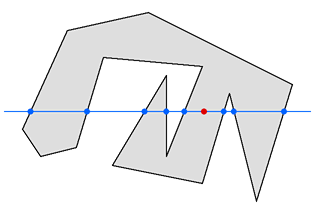
\includegraphics[width=8cm]{pinpolygon.png}
    \caption{Point in Polygon algorithm example }
    \label{fig-sample}
\end{figure}

Based on the Point-in-Polygon Algorithm(\url{http://alienryderflex.com/polygon/}), here is an example, the solution is to compare each side of the polygon to the Y (vertical) coordinate of the test point, and compile a list of nodes, where each node is a point where one side crosses the Y threshold of the test point. In this example, eight sides of the polygon cross the Y threshold, while the other six sides do not. Then, if there are an odd number of nodes on each side of the test point, then it is inside the polygon; if there are an even number of nodes on each side of the test point, then it is outside the polygon. In our example, there are five nodes to the left of the test point, and three nodes to the right. Since five and three are odd numbers, our test point is inside the polygon.
Then with more examples:
\begin{figure}[h!]
    \centering
    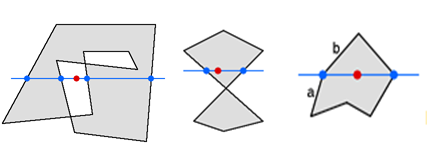
\includegraphics[width=12cm]{pinpolgonmoreexamples.png}
    \caption{More examples for Point in Polygon algorithm}
    \label{fig-sample}
\end{figure}

\end{itemize}